\section{Many-body localisation}
\subsection{Dummy}
\begin{frame}{Many-body localisation}
\begin{block}{\textbf{Isolated} quantum system, \textbf{strong interactions}, disorder or quasiperiodicity}
	\begin{enumerate}
		\item Usual: ergodic dynamics, transport, \textcolor{comp}{eigenstate thermalisation hypothesis (ETH)},
		\item Unusual: non-ergodicity, no transport, \textcolor{BostonBlue}{many-body localisation (MBL)}.
	\end{enumerate}
\end{block}

\begin{columns}
\begin{column}{0.5\textwidth}
\centering
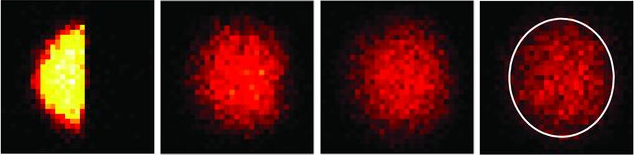
\includegraphics[width=0.9\columnwidth]{img/2_MBL/Imbalance_Choi_thermal}

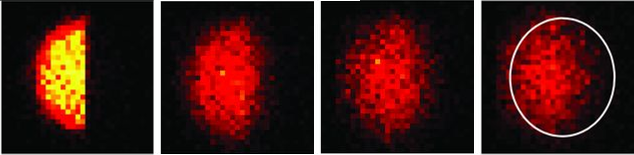
\includegraphics[width=0.9\columnwidth]{img/2_MBL/Imbalance_Choi}

[Choi \emph{et al} 16]
\end{column}
\begin{column}{0.5\textwidth}
\textbf{Experiments}: cold ions/atoms {\footnotesize[Schreiber \emph{et al} 15; Smith \emph{et al} 15; Bordia \emph{et al} 17]}.

\textbf{Motivations}:
\begin{itemize}
	\item ETH/MBL phase transition,
	\item MBL in more than 1D,
	\item Ingredients for MBL (this talk).
\end{itemize}
\end{column}
\end{columns}
\end{frame}

\begin{frame}{A model for MBL}
Chain of interacting spinless fermions (nb: no phonons):
\[
	H = \sum_{i=1}^L \left[ J (c_i^\dagger c_{i+1} + \text{h.c}) + \Delta n_i n_{i+1} - h_i n_i \right]
\]

\begin{columns}
\begin{column}{0.5\textwidth}
Disordered:
\centering
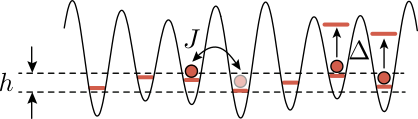
\includegraphics[height=2cm]{img/2_MBL/XXZ_cold_atoms}
\end{column}
%
\begin{column}{0.5\textwidth}
Quasiperiodic (this talk):
\centering
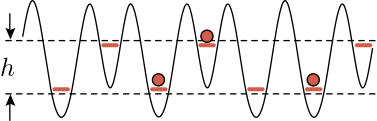
\includegraphics[height=2cm]{img/2_MBL/XXZ_QP_cold_atoms}
\end{column}
\end{columns}
Generic model: fermions, $\frac{1}{2}$ spins, hardcore bosons.

{
\centering
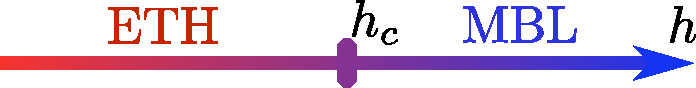
\includegraphics[width=0.5\textwidth]{img/2_MBL/arrow}

}
\end{frame}

\begin{frame}{MBL phenomenology}
\begin{columns}
\begin{column}{0.5\textwidth}
\centering
Phase diagram at $\Delta = 1$ {\footnotesize[Luitz \emph{et al} 15]}

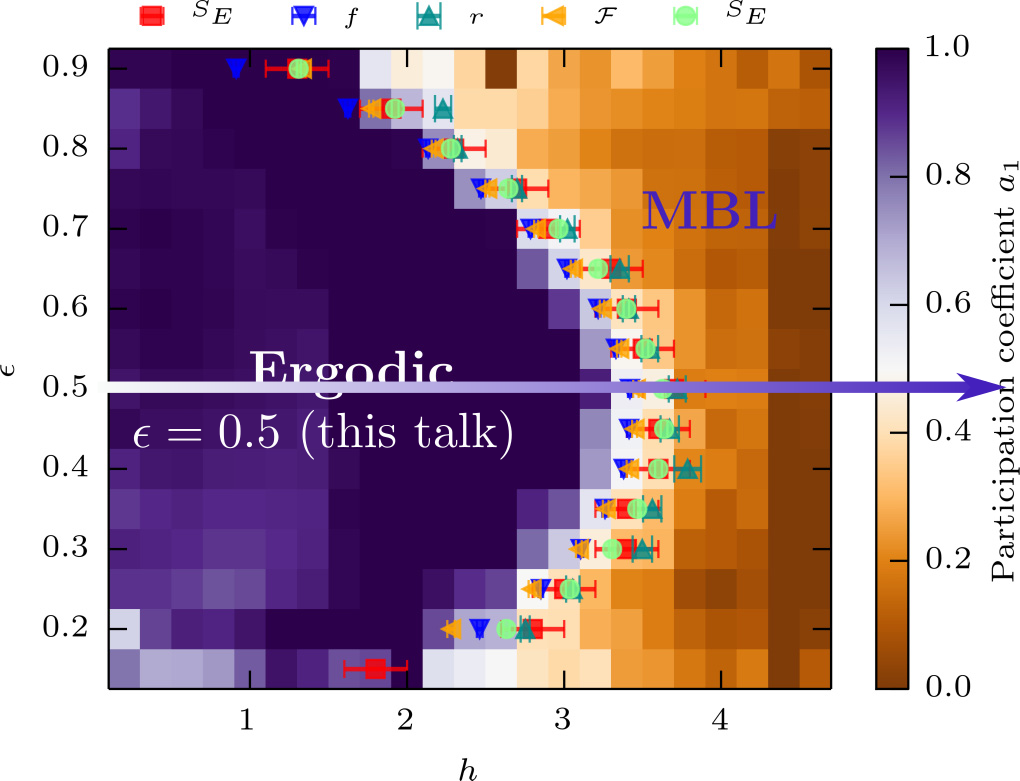
\includegraphics[width=0.75\textwidth]{img/2_MBL/edge2}
\end{column}
\begin{column}{0.5\textwidth}
\centering
Fermion density at $\epsilon = 0.5$
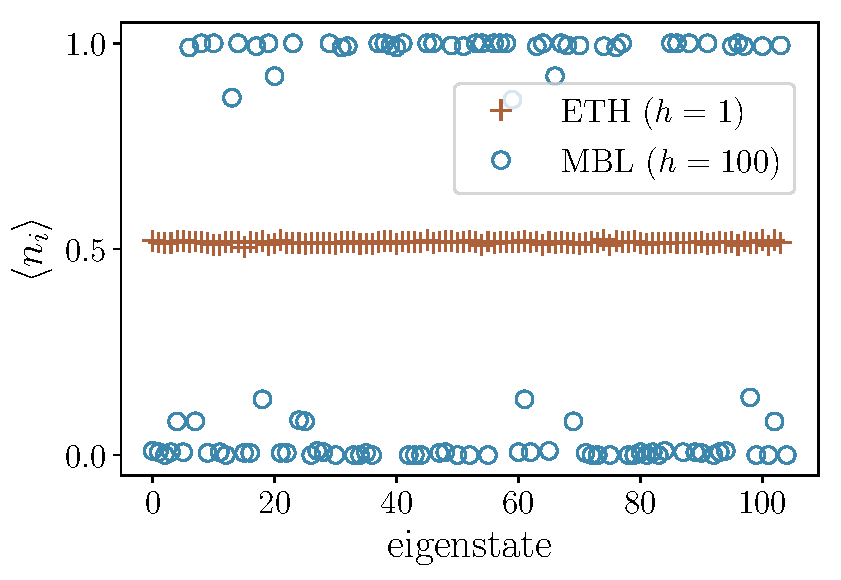
\includegraphics[width=0.8\textwidth]{img/2_MBL/local_observable}
\end{column}
\end{columns}
%%%%%%%%%%%%%%%%%%%%%%%%%%%%%%%%%%%%
\begin{columns}
\begin{column}{0.5\textwidth}
ETH:
\begin{itemize}
	\item Transport, thermal observables
	\item High entanglement
	\item Non-integrability
\end{itemize}
\end{column}
\begin{column}{0.5\textwidth}
MBL:
\begin{itemize}
	\item No transport, non-thermal observables
	\item Low entanglement
	\item Emergent integrability
\end{itemize}
\end{column}
\end{columns}
\end{frame}

\begin{frame}{Ingredients for MBL}
\begin{columns}
\begin{column}{0.65\textwidth}
Usually:
\begin{enumerate}
	\item $\Delta=0$: \textbf{localized} (random, Aubry-André potential)
	\item $\Delta \neq 0$: localization persists
\end{enumerate}
\end{column}
\begin{column}{0.35\textwidth}
\centering
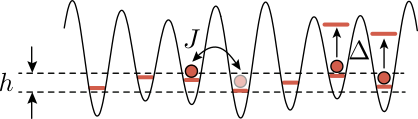
\includegraphics[width=\textwidth]{img/2_MBL/XXZ_cold_atoms}
\end{column}
\end{columns}
~\\
~\\

\begin{columns}
\begin{column}{0.65\textwidth}
This talk
\begin{enumerate}
	\item $\Delta=0$: \textbf{multifractal} (quasiperiodic potential)
	\item $\Delta\neq0$: localization appears
\end{enumerate}
\end{column}
\begin{column}{0.35\textwidth}
\centering
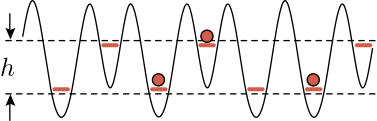
\includegraphics[width=\textwidth]{img/2_MBL/XXZ_QP_cold_atoms}
\end{column}
\end{columns}
~\\

\begin{block}{\textbf{Interest}}
\begin{itemize}
	\item MBL is \textbf{generic}
	\item Interplay between quasiperiodicity and MBL
\end{itemize}
\end{block}

\end{frame}